\section{Charging segments at their starting nodes}\label{sm:s:section}

We now allow an atom to start at any node of a tree. Its cost depends on
where it starts: masses on one branch add, whereas masses entering distinct
child subtrees combine in Euclidean norm. The resulting quotient norm has
a squared midpoint estimate. The proof matches opposite signed segments
at their first node outside a finite head and charges the discarded part
to the later of their two starting nodes.

\subsection{The cost and the completed space}

For each integer $n\ge1$, let $\mathcal T_n=\mathbb N^{\le n}$, including
its root $\varnothing$. Give nodes their component label, so the trees are
disjoint. Write $t\preceq v$ when $t$ is an initial segment of $v$, and
$[t,v]=\{s:t\preceq s\preceq v\}$. All scalars in this section are real.
For a nonnegative array $m$ on $\mathcal T_n$, define, upwards from the
leaves,
\begin{equation}\label{sm:s:cost}
 q_t(m)=m_t+\Bigl(\sum_{s\text{ child of }t}q_s(m)^2\Bigr)^{1/2},
 \qquad M_n(m)=q_{\varnothing}(m).
\end{equation}
Empty sums are zero; infinite values are allowed in this definition.
On the disjoint union $\mathcal T$ of the trees put
\[
 M(m)=\Bigl(\sum_{n\ge1}M_n(m|_{\mathcal T_n})^2\Bigr)^{1/2}.
\]
Thus $M_n$ is a cost for nonnegative start masses, before any vector norm
has been defined.

\begin{lemma}\label{sm:s:cost-properties}
The costs are monotone, positively homogeneous and subadditive. On
$\mathcal T_n$ they satisfy
\begin{equation}\label{sm:s:cost-comparisons}
 \|m\|_2\le M_n(m)
 \le\sum_{d=0}^{n}\|m|_{\mathbb N^d}\|_2
 \le\sqrt{n+1}\,\|m\|_2,
 \qquad
 \sum_{t\preceq v}m_t\le M_n(m).
\end{equation}
For nonnegative forest arrays of finite total cost,
\begin{equation}\label{sm:s:positive-energy}
 M(m+r)^2\ge M(m)^2+M(r)^2.
\end{equation}
\end{lemma}
\begin{proof}
Monotonicity and homogeneity follow directly by induction through the
levels. The same induction and the triangle inequality in $\ell_2$ give
subadditivity. Squaring~\eqref{sm:s:cost} and discarding its nonnegative
cross term proves the lower bound in~\eqref{sm:s:cost-comparisons}.
The $\ell_2$ norm of the $q_t$ on level $d$ is at most the $\ell_2$ norm of
the $m_t$ on that level plus the $\ell_2$ norm of the $q_s$ on level $d+1$.
Iterating gives the middle bound; Cauchy--Schwarz gives the last one.
Keeping only the child on the path to $v$ at each step gives the path
bound.

For the energy inequality, induction proves
$q_t(m+r)\ge(q_t(m)^2+q_t(r)^2)^{1/2}$. Indeed, let $A$ and $B$ be the
$\ell_2$ norms of the child values for $m$ and $r$. The induction
hypothesis gives
\[
 q_t(m+r)\ge m_t+r_t+\sqrt{A^2+B^2}
 \ge\sqrt{m_t^2+r_t^2}+\sqrt{A^2+B^2}
 \ge\sqrt{(m_t+A)^2+(r_t+B)^2}.
\]
The last inequality is the triangle inequality in $\mathbb R^2$.
Summing its square over the roots proves~\eqref{sm:s:positive-energy}.
These arguments apply to countably many children: all sums are
nonnegative, and the $\ell_2$ inequalities hold for finite partial sums
and then by monotone convergence. This also shows that each cost commutes
with increasing limits of nonnegative arrays.
\end{proof}

A segment representation on $\mathcal T_n$ is an array
$a=(a_{tv})_{t\preceq v}$ with start masses
\[
 m_t(a)=\sum_{v\succeq t}|a_{tv}|
 \quad\text{and}\quad M_n(m(a))<\infty.
\]
Its output is
\begin{equation}\label{sm:s:output}
 (Pa)_s=\sum_{t\preceq s}\sum_{v\succeq s}a_{tv}.
\end{equation}
Each coefficient $a_{tv}$ contributes its value on the entire segment
$[t,v]$. The sums at a fixed coordinate converge absolutely, by the path
bound in~\eqref{sm:s:cost-comparisons}.

\begin{proposition}\label{sm:s:space}
On $\ell_2(\mathcal T_n)$ the formula
\[
 \|x\|_{S,n}=\inf\{M_n(m(a)):Pa=x\}
\]
defines a complete reflexive norm, with
\begin{equation}\label{sm:s:norm-comparisons}
 \frac{\|x\|_2}{n+1}\le\|x\|_{S,n}
 \le\sqrt{n+1}\,\|x\|_2.
\end{equation}
Consequently
\[
 X_S=\Bigl(\bigoplus_{n\ge1}(\ell_2(\mathcal T_n),\|\cdot\|_{S,n})
       \Bigr)_{\ell_2}
\]
is a reflexive Banach space. Write $\|\cdot\|_S$ for its norm. Equivalently,
$\|x\|_S$ is the infimum of $M(m(a))$ over all forest representations of
$x$. Finite-support vectors are dense.
\end{proposition}
\begin{proof}
First we bound the output of a representation. Fix an output level $d$
and a start level $h\le d$. Segments starting at a single node $t$ of level
$h$ contribute total absolute mass at most $m_t(a)$ to level $d$; starts
at different nodes of level $h$ have disjoint descendants. Therefore the
$\ell_2$ norm of this part of the output is at most
$\|m(a)|_{\mathbb N^h}\|_2$. Summing over $h\le d$ bounds the norm on level
$d$ by $\sqrt{n+1}\,M_n(m(a))$. Summing the squares over $d$ gives
\begin{equation}\label{sm:s:output-bound}
 \|Pa\|_2\le(n+1)M_n(m(a)).
\end{equation}
Conversely, the singleton representation $a_{tt}=x_t$ has cost at most
$\sqrt{n+1}\|x\|_2$. This proves finiteness and the comparisons. Homogeneity
is immediate. Adding representations and using monotonicity and
subadditivity of the cost proves the triangle inequality; the lower
comparison proves definiteness. The norm is equivalent to the Hilbert
norm, and hence is complete and reflexive.

The countable $\ell_2$ sum is complete. Its dual is isometrically the
$\ell_2$ sum of the component duals: restriction of a functional gives
the component functionals, finite collections of approximate norming
vectors give the lower bound for their $\ell_2$ norm, and
Cauchy--Schwarz gives the reverse bound. Finite-component vectors are
dense, so restrictions determine the functional. Applying this
identification twice and using the reflexivity of every component proves
reflexivity of $X_S$.

A forest representation bounds each component norm by its component
cost, and therefore bounds $\|x\|_S$ by its total cost. Conversely, for
$\eta>0$ choose a representation in component $n$ with cost at most
$\|x|_{\mathcal T_n}\|_{S,n}+\eta2^{-n}$. Minkowski's inequality makes its
total cost less than $\|x\|_S+\eta$. Finally, finite support is dense in
each component by~\eqref{sm:s:norm-comparisons}, and finite-component
vectors are dense in the sum.
\end{proof}

We will keep separate entries on identical segments when convenient.
More precisely, one may use a countable list of signed segment weights
whose absolute start masses have finite cost. Combining entries on each
segment only decreases the start masses and gives a representation in
the preceding sense. Splitting a weight into pieces of the same sign
preserves the masses. These observations allow the matching argument
below without any assumption that an infimum is attained.

A subset of $\mathcal T$ is \emph{ancestral} if it contains every ancestor
of each of its nodes.

\begin{lemma}\label{sm:s:coordinates}
For every node $v$ and $x\in X_S$, $|x_v|\le\|x\|_S$. The coordinate vector
$e_v$ and every root-to-node path vector have norm one. If $C$ is a finite
ancestral subset of $\mathcal T$, then its coordinate projection $P_C$ is
contractive and $\|I-P_C\|\le2$. For a nonterminal node $t$, the sequence
of its child coordinate vectors is weakly null.
\end{lemma}
\begin{proof}
The absolute value of the output at $v$ is at most the sum of start
masses on the ancestor path to $v$, which is bounded by $M(m(a))$.
Take the infimum over representations. A singleton or a root-to-node
path has a representation of cost one, and its nonzero coordinate gives
the matching lower bound.

Restrict each representing segment to $C$. Since $C$ contains every
ancestor of its nodes, this restriction is empty or a segment with the
same start. The start masses cannot increase. Taking infima proves
$\|P_Cx\|_S\le\|x\|_S$; the bound for $I-P_C$ follows by the triangle
inequality. The child vectors lie in a fixed component and are weakly
null there, because its norm is equivalent to the Hilbert norm. They
remain weakly null under its inclusion in $X_S$.
\end{proof}

The unit path vectors in arbitrarily tall trees, together with their
weakly null unit increments, satisfy the hypotheses of
Lemma~\ref{lem:bounded-tree}. Thus $X_S$ admits no equivalent asymptotically
uniformly convex norm. More explicitly, if
$\alpha\|x\|_S\le N(x)\le\beta\|x\|_S$ and the modulus of $N$ were positive
at $t_0=\alpha/(2\beta)$, the lemma would extend a path with a factor
$1+\overline\delta_N(t_0)/4$ at every step. Its $N$ norm would eventually
exceed $\beta$, although every such path has $\|\cdot\|_S$ norm one.

\subsection{A squared estimate across a finite cut}

The next theorem is the geometric estimate supplied by this model.
Unlike a root-path cost, the present cost records the starting node of
each segment. Removing one of two opposite crossing segments saves
the mass charged at its later start. The positive energy
inequality then turns that saved mass into a squared gain.

\begin{theorem}\label{thm:segment-start-tail}
Let $C$ be a finite ancestral subset of $\mathcal T$. If $p\in X_S$ is
supported in $C$ and $y\in X_S$ satisfies $y|_C=0$, then
\begin{equation}\label{sm:s:tail}
 \max\{\|p+y\|_S,\|p-y\|_S\}^2
 \ge\|p\|_S^2+\frac{\|y\|_S^2}{64}.
\end{equation}
The conclusion includes $C=\varnothing$, $p=0$ and $y=0$.
\end{theorem}
\begin{figure}[tb]
\centering
\begin{minipage}[t]{0.48\textwidth}
\centering
\textbf{(a) Recover the center}\par\smallskip
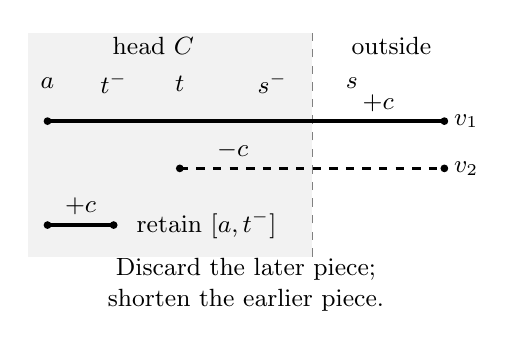
\begin{tikzpicture}[x=0.84cm,y=0.8cm,font=\small]
 \fill[black!5] (-0.3,0.25) rectangle (4,3.8);
 \draw[dashed,gray] (4,0.25)--(4,3.8);
 \node at (1.6,3.6) {head $C$};
 \node at (5.2,3.6) {outside};
 \foreach \x/\name in {0/a,1/{t^-},2/t,3.4/{s^-},4.6/s}
  {\node at (\x,3.0) {$\name$};}
 \draw[very thick] (0,2.4)--(6,2.4);
 \fill (0,2.4) circle (1.4pt); \fill (6,2.4) circle (1.4pt);
 \node[above] at (5,2.4) {$+c$};
 \node[right] at (6,2.4) {$v_1$};
 \draw[very thick,dashed] (2,1.65)--(6,1.65);
 \fill (2,1.65) circle (1.4pt); \fill (6,1.65) circle (1.4pt);
 \node[above] at (2.8,1.65) {$-c$};
 \node[right] at (6,1.65) {$v_2$};
 \draw[very thick] (0,0.75)--(1,0.75);
 \fill (0,0.75) circle (1.4pt); \fill (1,0.75) circle (1.4pt);
 \node[above] at (0.5,0.75) {$+c$};
 \node[right,align=left] at (1.2,0.75) {retain $[a,t^-]$};
 \node[align=center] at (3,-0.2) {Discard the later piece;\\shorten the earlier piece.};
\end{tikzpicture}
\end{minipage}\hfill
\begin{minipage}[t]{0.48\textwidth}
\centering
\textbf{(b) Recover one exterior piece}\par\smallskip
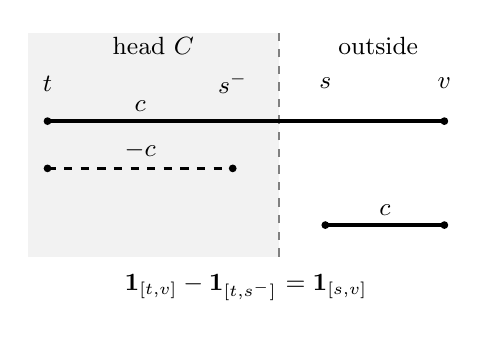
\begin{tikzpicture}[x=0.84cm,y=0.8cm,font=\small]
 \fill[black!5] (-0.3,0.25) rectangle (3.5,3.8);
 \draw[dashed,gray] (3.5,0.25)--(3.5,3.8);
 \node at (1.6,3.6) {head $C$};
 \node at (5.0,3.6) {outside};
 \foreach \x/\name in {0/t,2.8/{s^-},4.2/s,6/v}
  {\node at (\x,3.0) {$\name$};}
 \draw[very thick] (0,2.4)--(6,2.4);
 \fill (0,2.4) circle (1.4pt); \fill (6,2.4) circle (1.4pt);
 \node[above] at (1.4,2.4) {$c$};
 \draw[very thick,dashed] (0,1.65)--(2.8,1.65);
 \fill (0,1.65) circle (1.4pt); \fill (2.8,1.65) circle (1.4pt);
 \node[above] at (1.4,1.65) {$-c$};
 \draw[very thick] (4.2,0.75)--(6,0.75);
 \fill (4.2,0.75) circle (1.4pt); \fill (6,0.75) circle (1.4pt);
 \node[above] at (5.1,0.75) {$c$};
 \node[align=center] at (3,-0.2) {$\mathbf1_{[t,v]}-\mathbf1_{[t,s^-]}$
  \strut$=\mathbf1_{[s,v]}$};
\end{tikzpicture}
\end{minipage}
\caption{Segment matching in the representative case
$a\prec t\preceq s^-$, where $a$ and $t$ are the earlier and later
starts and $s$ is the first node outside the head. Each row represents
a segment; its labels through $s$ refer to the common ancestor chain.
In (a), the displayed signs are opposite coefficient signs, with
$c>0$; they are independent of the $+$ and $-$ endpoint-origin labels.
In (b), a piece from the $+$ endpoint can have either sign of $c$.
Its exterior is reproduced using at most two segments starting at $t$.
The proof also covers coincident starts, $t=s$, and roots outside $C$.}
\label{fig:segment-matching}
\end{figure}

\begin{proof}
Fix $\eta>0$ and put
$R=\max\{\|p+y\|_S,\|p-y\|_S\}+\eta$. Choose representations of $p+y$
and $p-y$ of cost at most $R$. Halve every coefficient and concatenate
the two lists, retaining the labels $+$ and $-$ that record their
origins. These labels are independent of the signs of the coefficients.
The combined list has output $p$ and start mass $m$ with $M(m)\le R$.
Figure~\ref{fig:segment-matching} illustrates the two uses of a matched pair.

A first node outside $C$ means a node $s\notin C$ whose parent lies in
$C$, or a root outside $C$. Every segment is then of exactly one of
three kinds: it lies wholly in $C$; it contains one first node outside
$C$; or its start lies strictly below a first node outside $C$.
The second kind includes segments starting at that first node.
At each such $s$, match the positive and
negative weights of all segments containing $s$ in pieces of equal
absolute weight. Their total positive and total negative masses are
finite and equal, since their sum is the output $p_s=0$. For completeness,
place the positive weights consecutively on an interval of their total
length, do the same with the absolute negative weights, and use the
intersections of these intervals as matching pieces. This produces a
countable matching that uses every weight. A segment contains at most
one first node outside $C$, so the matchings do not interfere.

In each matched pair, both starts are ancestors of its first outside
node $s$. Call the piece with deeper start the later piece, breaking a
tie arbitrarily. Define $r_t$ to be the sum of the sizes of later pieces
starting at $t$, together with the sizes of all original pieces starting
strictly below a first node outside $C$. These are disjoint portions of
the list; hence $0\le r\le m$.

We first recover $p$ at cost at most $M(m-r)$. Delete all pieces starting
strictly below a first outside node. For a matched pair with coincident
starts, discard both pieces. Otherwise discard the later piece and
shorten the earlier piece to end immediately before the later start.
The remaining part
lies in $C$. On $C$ the removed overlapping parts had equal opposite
coefficients and therefore canceled. Segments wholly inside $C$ are
unchanged. The modified list consequently represents $p$, and its start
masses are at most $m-r$. By~\eqref{sm:s:positive-energy},
\begin{equation}\label{sm:s:saved-mass}
 \|p\|_S^2+M(r)^2\le M(m-r)^2+M(r)^2\le M(m)^2.
\end{equation}

It remains to control $y$ by the saved mass. The output of the $+$ list
outside $C$ is $y/2$. We represent it using start masses at most $4r$.
Include each $+$ piece starting strictly below a first outside node
without change. For a $+$ piece in a pair at $s$, let $t$ be the pair's
later start and $v$ the endpoint of this piece. Replace its exterior part
by the segment $[t,v]$ with its original coefficient. If $t\in C$, also
include the segment from $t$ to the parent of $s$ with the opposite
coefficient. These two segments leave precisely the desired output
from $s$ to $v$. If $t=s$, no subtraction is needed. Each pair has at most
two $+$ pieces, and each uses at most two segments of the matched size,
all starting at $t$. Their total start mass is therefore at most four
times the later piece's mass. No segment wholly in $C$ is needed. Thus
\begin{equation}\label{sm:s:tail-recovery}
 \|y\|_S\le2M(4r)=8M(r).
\end{equation}

All the modified lists are legitimate: their absolute start masses have
finite cost, and each coordinate has only finitely many ancestors.
Combining~\eqref{sm:s:saved-mass} and~\eqref{sm:s:tail-recovery} gives
$\|p\|_S^2+\|y\|_S^2/64\le R^2$. Finally let $\eta\downarrow0$.
\end{proof}

\begin{corollary}\label{sm:s:midpoint-consequence}
For every $x\in X_S$ with $\|x\|_S=1$, every $t>0$ and every $\varepsilon>0$
there is a closed finite-codimensional subspace $F\subset X_S$ such that
\[
 \inf_{\substack{y\in F\\\|y\|_S=1}}
 \max\{\|x+ty\|_S,\|x-ty\|_S\}
 \ge\sqrt{1+t^2/64}-\varepsilon.
\]
In particular, define the maximum form of the asymptotic midpoint modulus
by
\[
 \delta^{\max}_{X_S}(t)=
 \inf_{\|x\|_S=1}\sup_{\substack{F\subset X_S\text{ closed}\\\dim(X_S/F)<\infty}}
 \inf_{\substack{y\in F\\\|y\|_S\ge1}}
 \bigl(\max_{\pm}\|x\pm ty\|_S-1\bigr).
\]
Then $\delta^{\max}_{X_S}(t)\ge\sqrt{1+t^2/64}-1$.
\end{corollary}
\begin{proof}
Choose a finite-support $p$ arbitrarily close to $x$, let $C$ be its finite
ancestral closure and set $F=\ker P_C$. Theorem~\ref{thm:segment-start-tail}
gives, uniformly for $y\in F$ with $\|y\|_S\ge1$,
\[
 \max_{\pm}\|x\pm ty\|_S
 \ge\sqrt{\|p\|_S^2+t^2/64}-\|x-p\|_S.
\]
As $\|x-p\|_S\to0$, the right side tends to
$\sqrt{1+t^2/64}$. Coordinate continuity makes $F$ closed and
finite-codimensional, proving the assertion.
\end{proof}

\section{Incomparable segments}
\label{sm:i:section}

In this section, arrays are tested by families of segments in which every
node of one segment is incomparable with every node of another.  The resulting dual space has unit root paths of
arbitrarily large finite height. When both endpoints lie in the unit ball,
a midpoint close to the unit sphere forces small displacement beyond any
finite prefix supporting that midpoint. We prove the latter assertion by replacing the
coefficients of segment atoms with the sums of a norming test along their
segments.  Opposite signs can then be controlled by shortening segments
without violating their incomparability.

\subsection{The norm and its dual atoms}

For an integer $h\geq1$, let $T_h=\mathbb N^{\leq h}$, including the empty
sequence as its root, and take disjoint copies when forming
$\mathcal T=\bigsqcup_{h\geq1}T_h$.
Nodes in the same tree are ordered by extension, denoted by $s\preceq t$;
nodes in different trees are incomparable.  If $s\preceq t$, the segment
$[s,t]$ consists of every node between $s$ and $t$, including both
endpoints.  A finite family $(S_i)_{i=1}^m$ of nonempty segments is
\emph{incomparable} if, for $i\ne j$, every node of $S_i$ is incomparable
with every node of $S_j$.  In particular, the segments are disjoint, but
disjointness alone is not this condition.

For a finitely supported real array $g$ on $\mathcal T$, set
\begin{equation}
 \|g\|_{Y_{\mathrm I}}
 =\sup_{(S_i)\text{ incomparable}}
   \left(\sum_{i=1}^m
     \left|\sum_{v\in S_i}g(v)\right|^2\right)^{1/2},
 \label{sm:i:norm}
\end{equation}
and let $Y_{\mathrm I}$ be its completion.  This is a finite norm on
$c_{00}(\mathcal T)$: the triangle inequality follows from the Euclidean
triangle inequality, singleton tests separate points, and disjointness
bounds every test by $\sum_v|g(v)|$.
Each coordinate and each finite segment evaluation extends continuously
to $Y_{\mathrm I}$.  Formula~\eqref{sm:i:norm} remains valid in the
completion.  Indeed, the supremum of the extended tests is at most the
completion norm and is Lipschitz with constant one; approximation by
finitely supported arrays gives the reverse inequality.

Quadratic aggregation over incomparable segment families also appears
in the $\ell_2$-Baire-sum construction of Argyros and Dodos
\cite[author version, Section~4.1]{ArgyrosDodos2007}. There each segment
contributes the norm of a sum in a Schauder tree basis; here it contributes
the absolute scalar sum in~\eqref{sm:i:norm}.

\begin{proposition}\label{sm:i:reflexivity}
Let $Y_{\mathrm I,h}$ be the completion of the arrays supported on $T_h$
in the norm~\eqref{sm:i:norm}.  Then
\begin{equation}
 \frac{\|g\|_2}{\sqrt{h+1}}
 \leq\|g\|_{Y_{\mathrm I,h}}
 \leq\sqrt{h+1}\,\|g\|_2,
 \qquad g\in c_{00}(T_h),
 \label{sm:i:hilbert}
\end{equation}
and
\[
 Y_{\mathrm I}=\left(\bigoplus_{h\geq1}Y_{\mathrm I,h}\right)_{\ell_2}.
\]
Both $Y_{\mathrm I}$ and $X_{\mathrm I}:=Y_{\mathrm I}^*$ are reflexive.
\end{proposition}

\begin{proof}
At each fixed level of $T_h$, the singleton segments form an incomparable
family.  Hence the squared norm of $g$ dominates the sum of $|g(v)|^2$
over that level.  Summing over the $h+1$ levels gives the lower bound
in~\eqref{sm:i:hilbert}.  For the upper bound, every segment has at most
$h+1$ nodes, so Cauchy--Schwarz and disjointness give
\[
 \sum_i\left|\sum_{v\in S_i}g(v)\right|^2
 \leq(h+1)\sum_i\sum_{v\in S_i}|g(v)|^2
 \leq(h+1)\|g\|_2^2.
\]
Thus $Y_{\mathrm I,h}$ is isomorphic to the Hilbert space $\ell_2(T_h)$
and is reflexive.

A test family separates into families on the individual trees.  Conversely,
the union of finitely many such families, one in each of distinct trees,
is incomparable.  Choosing each component family arbitrarily close to
its supremum proves
\[
 \|g\|_{Y_{\mathrm I}}^2
 =\sum_h\|g|_{T_h}\|_{Y_{\mathrm I,h}}^2
\]
for finitely supported $g$, and then the asserted sum decomposition
follows by completion.
For completeness, the dual of an $\ell_2$-sum of Banach spaces is the
$\ell_2$-sum of their duals: Cauchy--Schwarz bounds the sum of the
pairings, while finitely many nearly norming component vectors with
suitable scalar weights give the opposite norm inequality.  Restrictions
to the components determine a functional by density.  Applying this
description twice, componentwise reflexivity shows that the canonical
map into the bidual is onto.  Thus $Y_{\mathrm I}$ is reflexive, as is
its dual $X_{\mathrm I}$.
\end{proof}

Write $e_v\in X_{\mathrm I}$ for evaluation at $v$, and put
$z_S=\sum_{v\in S}e_v$, with $z_\varnothing=0$.  We denote the dual norm
by $\|\cdot\|_{\mathrm I}$.  The coordinate evaluations are linearly
independent, so $X_{\mathrm I}$ is infinite dimensional.  An \emph{atom}
is a vector together with a representation
\begin{equation}
 A=\sum_{i=1}^m a_i z_{S_i},
 \qquad \sum_{i=1}^m a_i^2\leq1,
 \qquad (S_i)_{i=1}^m\text{ incomparable}.
 \label{sm:i:atoms}
\end{equation}
The representation will matter when its coefficients are replaced below.

\begin{lemma}\label{sm:i:atom-hull}
The unit ball of $X_{\mathrm I}$ is the norm-closed convex hull of the
atoms~\eqref{sm:i:atoms}.  In particular, finite linear combinations of
the coordinate evaluations are dense in $X_{\mathrm I}$.
\end{lemma}

\begin{proof}
Every atom has norm at most one, by Cauchy--Schwarz
and~\eqref{sm:i:norm}, and for every $g\in Y_{\mathrm I}$,
\[
 \sup_{A\text{ atom}} A(g)=\|g\|_{Y_{\mathrm I}}.
\]
If the closed convex hull of the atoms missed a point of the dual unit
ball, Hahn--Banach separation would give a separating functional in
$X_{\mathrm I}^*=Y_{\mathrm I}$, using Proposition~\ref{sm:i:reflexivity}.
The displayed identity rules out such a separation.  Each atom has
finite support, which gives the density assertion.
\end{proof}

\subsection{Unit paths and finite prefixes}

The root paths give the one-sided obstruction; finite prefixes will
separate the head of a midpoint from its remaining coordinates.
For $s\in T_h$, define
\[
 v_s=z_{[\varnothing_h,s]},
\]
where $\varnothing_h$ denotes the root of that copy of $T_h$.
Each $v_s$ is an atom of norm one: its norm is at most one by
Lemma~\ref{sm:i:atom-hull}, and testing it against the array which equals
one at $s$ and zero elsewhere gives the reverse inequality.  The same
argument gives $\|e_t\|_{\mathrm I}=1$ for every node $t$.
If $|s|<h$ and $t_j=s^\frown j$, then
\begin{equation}
 v_{t_j}=v_s+e_{t_j},\qquad
 \|v_s\|_{\mathrm I}=\|e_{t_j}\|_{\mathrm I}=1,
 \qquad e_{t_j}\longrightarrow0\text{ weakly}.
 \label{sm:i:paths}
\end{equation}
To verify weak convergence, singleton tests at the children show that
$\sum_j|g(t_j)|^2\leq\|g\|_{Y_{\mathrm I}}^2$ for each
$g\in Y_{\mathrm I}$.  Thus $g(t_j)\to0$, and these are all the
functionals on $X_{\mathrm I}$ by reflexivity.

\begin{corollary}\label{sm:i:auc-obstruction}
The real reflexive space $X_{\mathrm I}$ admits no equivalent
asymptotically uniformly convex norm.
\end{corollary}

\begin{proof}
The trees~\eqref{sm:i:paths} exist at every finite height and satisfy
Lemma~\ref{lem:bounded-tree} with path bounds and increment lower bound
all equal to one.  More explicitly, for an equivalent norm $N$ with
$a\|u\|_{\mathrm I}\leq N(u)\leq b\|u\|_{\mathrm I}$, that lemma
uses $t_0=a/(2b)$.  If
$\delta=\overline\delta_N(t_0)>0$, its finite-codimensional approximation
and convexity argument selects a child at every nonterminal node for
which
\[
 N(v_{t_j})\geq (1+\delta/4)N(v_s).
\]
Iteration to height $h$ gives
$a(1+\delta/4)^h\leq b$, a contradiction for sufficiently large $h$.
\end{proof}

A set $E\subset\mathcal T$ is \emph{prefix closed} if it contains every
ancestor of each of its nodes, within that node's tree.  Let $P_E$ be
coordinate restriction to $E$, and let $Q_E=I-P_E$.

\begin{lemma}\label{sm:i:projections}
For every finite prefix-closed $E$, both $P_E$ and $Q_E$ act
contractively on $Y_{\mathrm I}$ and, by adjoints, on $X_{\mathrm I}$.
On $X_{\mathrm I}$, $P_E$ has finite rank and retains exactly the
coordinates indexed by $E$.  For every $x\in X_{\mathrm I}$ and every
$\eta>0$, there is such an $E$ with $\|Q_E x\|_{\mathrm I}<\eta$.
\end{lemma}

\begin{proof}
The nonempty intersections of an incomparable segment family with $E$
are again incomparable segments; the same is true of the portions
outside $E$.  Here prefix closure ensures that a segment is cut into
an initial part and a terminal part.  Applying these restricted tests to
the original array proves both contraction inequalities on
$Y_{\mathrm I}$, first on finite arrays and then on the completion.
The adjoints are contractions and act as the stated coordinate
projections on each $e_v$, hence on $X_{\mathrm I}$ by
Lemma~\ref{sm:i:atom-hull}.  The range of $P_E$ is contained in the span
of the finitely many $e_v$ with $v\in E$.
Finally, approximate $x$ by a finitely supported vector and let $E$
contain its support and all its ancestors.  The contraction bound for
$Q_E$ gives the last assertion.
\end{proof}

\subsection{Replacing coefficients and controlling cancellation}

The following estimate is uniform in the finite prefix and allows an
arbitrary displacement.  Its tail-supported case is the symmetric
splitting estimate for this model.

\begin{theorem}\label{sm:i:tail-estimate}
Let $E\subset\mathcal T$ be finite and prefix closed.  If
$x,y\in X_{\mathrm I}$ satisfy
\[
 P_E x=x,\qquad \|x+y\|_{\mathrm I}\leq1,
 \qquad \|x-y\|_{\mathrm I}\leq1,
\]
then
\begin{equation}
 \|Q_Ey\|_{\mathrm I}
 \leq (\sqrt2+\sqrt6)\sqrt{1-\|x\|_{\mathrm I}}.
 \label{sm:i:tail-bound}
\end{equation}
In particular, if $Q_Ey=y$, the same bound holds for $\|y\|_{\mathrm I}$.
\end{theorem}

\begin{proof}
Convexity gives $\|x\|_{\mathrm I}\leq1$.
Choose $f\in Y_{\mathrm I}$ supported on $E$ such that
\[
 \|f\|_{Y_{\mathrm I}}\leq1,
 \qquad x(f)=\|x\|_{\mathrm I}.
\]
Indeed, Hahn--Banach gives a norming element of $X_{\mathrm I}^*$;
reflexivity identifies it with an element of $Y_{\mathrm I}$, and
applying $P_E$ preserves its pairing with $x$ without increasing its
norm.  If $x=0$, we may simply take $f=0$.

For an atom with representation~\eqref{sm:i:atoms}, define
\[
 p_i^A=z_{S_i}(f),\qquad
 d(A)=1-A(f)=1-\sum_i a_i p_i^A\geq0.
\]
Both coefficient vectors $(a_i)$ and $(p_i^A)$ have Euclidean norm at
most one.  The identity
\[
 2d(A)=\sum_i(a_i-p_i^A)^2
       +\left(1-\sum_i a_i^2\right)
       +\left(1-\sum_i(p_i^A)^2\right)
\]
therefore gives
\begin{equation}
 \sum_i(a_i-p_i^A)^2\leq2d(A),
 \qquad 1-\sum_i(p_i^A)^2\leq2d(A).
 \label{sm:i:defect}
\end{equation}
Replace the coefficients on the terminal pieces by setting
\[
 \widehat A=\sum_i p_i^A z_{S_i\setminus E}.
\]
Those nonempty terminal pieces remain incomparable.  The atom norm
bound and~\eqref{sm:i:defect} imply
\begin{equation}
 \|\widehat A-Q_EA\|_{\mathrm I}\leq\sqrt{2d(A)}.
 \label{sm:i:replacement}
\end{equation}

Let $\mathcal R$ be the minimal nodes of $\mathcal T\setminus E$.
They form an antichain and their descendant subtrees partition the
complement.  If $p_i^A\ne0$ and $S_i\setminus E$ is nonempty, the original segment
meets $E$ and exits it through exactly one $q\in\mathcal R$.
For a fixed $q$, at most one segment in an incomparable family can do
this, since two such segments would both contain $q$.  We may write
\begin{equation}
 \widehat A=\sum_{q\in\mathcal R}r_q^A z_{[q,t_q^A]}.
 \label{sm:i:exits}
\end{equation}
Only finitely many coefficients are nonzero.  When $r_q^A\ne0$, let
$s_q^A\in E$ be the starting node of the original segment and let
$t_q^A\succeq q$ be its terminal node.  Then $r_q^A$ is the sum of $f$
from $s_q^A$ to the predecessor of $q$.  For zero coefficients choose
$t_q^A=q$; no starting node is needed.

We next show that opposite coefficients in two atoms consume their
norming defects:
\begin{equation}
 \sum_{q:\,r_q^Ar_q^{A'}<0}|r_q^Ar_q^{A'}|
 \leq \frac12\left(1-\sum_i(p_i^A)^2
                  +1-\sum_i(p_i^{A'})^2\right)
 \leq d(A)+d(A').
 \label{sm:i:cancellation}
\end{equation}
For any exit occurring in this sum, the two starting nodes lie on the
same ancestor path of $q$.  They are distinct, since identical starts
would give identical sums of $f$, rather than opposite signs.
Consider first the exits for which $s_q^A\prec s_q^{A'}$.
Shorten the corresponding segment of $A$ to the interval from $s_q^A$
to the predecessor of $s_q^{A'}$.  This interval is nonempty and is a
subsegment of the original segment.  Distinct exits correspond to
distinct segments, so all these shortenings can be made simultaneously.
Every modified family is still incomparable.  Its corresponding
squared evaluation changes from $(r_q^A)^2$ to
$(r_q^A-r_q^{A'})^2$, an increase of
\[
 (r_q^{A'})^2+2|r_q^Ar_q^{A'}|
 \geq2|r_q^Ar_q^{A'}|.
\]
All its squared evaluations sum to at most one.  Thus the sum of these
products is at most $\tfrac12(1-\sum_i(p_i^A)^2)$.
For the exits with the opposite ordering, shorten the segments of $A'$
instead and obtain the other half of~\eqref{sm:i:cancellation}.
The final inequality follows from~\eqref{sm:i:defect}.

We have controlled the replacement error for one atom and opposite
exit coefficients for two atoms.  It remains to apply these facts to
convex combinations approximating the two endpoints $x+y$ and $x-y$.
Fix $\varepsilon>0$.  By Lemma~\ref{sm:i:atom-hull}, choose a finite
probability distribution of atoms for each endpoint whose mean differs
from that endpoint in norm by at most $\varepsilon$.  Choose
$\sigma\in\{-1,1\}$ with equal probabilities, then choose $A$ from the
distribution for $x+\sigma y$.  Consequently
\[
 \|\mathbb E A-x\|_{\mathrm I}\leq\varepsilon,
 \qquad
 \|\mathbb E(\sigma A)-y\|_{\mathrm I}\leq\varepsilon,
 \qquad
 0\leq\bar d:=\mathbb E d(A)
 \leq1-\|x\|_{\mathrm I}+\varepsilon.
\]
Contractivity of $Q_E$, the identity $Q_Ex=0$, and
Cauchy--Schwarz applied to~\eqref{sm:i:replacement} give
\begin{equation}
 \|\mathbb E\widehat A\|_{\mathrm I}
 \leq\varepsilon+\sqrt{2\bar d},
 \qquad
 \|\mathbb E(\sigma\widehat A)-Q_Ey\|_{\mathrm I}
 \leq\varepsilon+\sqrt{2\bar d}.
 \label{sm:i:mixture-errors}
\end{equation}

Put $m_q=\mathbb E r_q^A$ and $b_q=\mathbb E|r_q^A|$.
Apply~\eqref{sm:i:cancellation} to independent copies $A,A'$ of the
unconditional atom distribution.  With $r_+=\max(r,0)$ and
$r_-=\max(-r,0)$, independence gives
\[
 2\sum_q\mathbb E[(r_q^A)_+]\,\mathbb E[(r_q^A)_-]
 \leq2\bar d.
\]
Since $b_q^2-m_q^2=4\mathbb E[(r_q^A)_+]\,\mathbb E[(r_q^A)_-]$,
\begin{equation}
 \sum_q b_q^2\leq\sum_qm_q^2+4\bar d.
 \label{sm:i:unsigned-mass}
\end{equation}
At this fixed $\varepsilon$, the distributions are finite and their
atoms have finite support.  Thus all sums of $m_q$ and $b_q$ above are
finite, even though $\mathcal R$ can be infinite.

An array supported on the antichain $\mathcal R$ has
$Y_{\mathrm I}$-norm equal to its Euclidean norm: a segment meets at
most one of its support nodes, and singleton segments realize the
Euclidean test.  The coefficient of $\mathbb E\widehat A$ at $q$ is
$m_q$, so duality gives
\begin{equation}
 \left(\sum_qm_q^2\right)^{1/2}
 \leq\|\mathbb E\widehat A\|_{\mathrm I}.
 \label{sm:i:signed-mass}
\end{equation}
For $g\in Y_{\mathrm I}$ with $\|g\|_{Y_{\mathrm I}}\leq1$, define
\[
 L_q=\sup_{t\succeq q}|z_{[q,t]}(g)|.
\]
For each finite subset of exits, choose segments approaching these
suprema.  The chosen segments are incomparable, so their squared
evaluations sum to at most one.  Passing to the suprema and then taking
the supremum over finite subsets proves $\sum_qL_q^2\leq1$;
no supremum need be attained.  It follows that
\[
 |\mathbb E(\sigma\widehat A)(g)|
 \leq\sum_qb_qL_q
 \leq\left(\sum_qb_q^2\right)^{1/2}.
\]
Taking the supremum over $g$, and
using~\eqref{sm:i:mixture-errors}--\eqref{sm:i:signed-mass}, yields
\[
 \|Q_Ey\|_{\mathrm I}
 \leq\varepsilon+\sqrt{2\bar d}
   +\left((\varepsilon+\sqrt{2\bar d})^2+4\bar d\right)^{1/2}.
\]
The right-hand side is increasing in $\bar d$.  Substitute
$\bar d\leq1-\|x\|_{\mathrm I}+\varepsilon$ and let
$\varepsilon\downarrow0$.  The two limiting contributions are
$\sqrt{2(1-\|x\|_{\mathrm I})}$ and
$\sqrt{6(1-\|x\|_{\mathrm I})}$, proving~\eqref{sm:i:tail-bound}.
\end{proof}

\subsection{Separated midpoint families}

The next corollary removes the finite-prefix condition on the center:
if $x\pm u_j$ lie in the unit ball for an infinite separated family
$(u_j)$, then the norm of the common midpoint $x$ is bounded away from one.

\begin{corollary}\label{sm:i:separated-midpoints}
Let $0<c\leq1$ and let $x,u_j\in X_{\mathrm I}$, $j\in\mathbb N$,
satisfy
\[
 \|x+u_j\|_{\mathrm I},\ \|x-u_j\|_{\mathrm I}\leq1,
 \qquad \|u_j-u_k\|_{\mathrm I}\geq2c\quad(j\ne k).
\]
Then, with $K=\sqrt2+\sqrt6$,
\begin{equation}
 \|x\|_{\mathrm I}\leq1-(c/K)^2<1.
 \label{sm:i:separation-bound}
\end{equation}
\end{corollary}

\begin{proof}
Fix $0<\eta<c$ and use Lemma~\ref{sm:i:projections} to choose $E$ with
$\|Q_Ex\|_{\mathrm I}<\eta$.  The sequence $(u_j)$ is bounded, since
$u_j=((x+u_j)-(x-u_j))/2$.  The range of $P_E$ is finite dimensional,
so there are distinct $j,k$ such that, for
$w=(u_j-u_k)/2$, one has $\|P_Ew\|_{\mathrm I}<\eta$.
The separation assumption gives $\|w\|_{\mathrm I}\geq c$.
Moreover, $x+w$ is the midpoint of $x+u_j$ and $x-u_k$, and $x-w$ is
the midpoint of the other two endpoints.  Hence
$\|x\pm w\|_{\mathrm I}\leq1$.  Therefore
\[
 \|P_Ex\pm Q_Ew\|_{\mathrm I}\leq1+2\eta,
 \qquad \|Q_Ew\|_{\mathrm I}\geq c-\eta.
\]
Apply Theorem~\ref{sm:i:tail-estimate} after dividing both vectors by
$1+2\eta$:
\[
 \frac{c-\eta}{1+2\eta}
 \leq K\sqrt{1-\frac{\|P_Ex\|_{\mathrm I}}{1+2\eta}}.
\]
Since $\|P_Ex-x\|_{\mathrm I}<\eta$, letting $\eta\downarrow0$ gives
$ c\leq K\sqrt{1-\|x\|_{\mathrm I}}$, which is
\eqref{sm:i:separation-bound}.
\end{proof}
